\cleardoublepage
\chapter{外文原文}

% Insert pdf version of original document
% Place the pdf under `/figure/`

\section*{Abstract}

\par The goal of precipitation nowcasting is to predict the future rainfall intensity in a local region over a relatively short period of time. Very few previous studies have examined this crucial and challenging weather forecasting problem from the machine learning perspective. In this paper, we formulate precipitation nowcasting as a spatiotemporal sequence forecasting problem in which both the input and the prediction target are spatiotemporal sequences. By extending the fully connected LSTM (FC-LSTM) to have convolutional structures in both the input-to-state and state-to-state transitions, we propose the convolutional LSTM (ConvLSTM) and use it to build an end-to-end trainable model for the precipitation nowcasting problem. Experiments show that our ConvLSTM network captures spatiotemporal correlations better and consistently outperforms FC-LSTM and the state-of-theart operational ROVER algorithm for precipitation nowcasting.

\section{Introduction}

\par Nowcasting convective precipitation has long been an important problem in the field of weather forecasting. The goal of this task is to give precise and timely prediction of rainfall intensity in a local region over a relatively short period of time (e.g., 0-6 hours). It is essential for taking such timely actions as generating society-level emergency rainfall alerts, producing weather guidance for airports, and seamless integration with a longer-term numerical weather prediction (NWP) model. Since the forecasting resolution and time accuracy required are much higher than other traditional forecasting tasks like weekly average temperature prediction, the precipitation nowcasting problem is quite challenging and has emerged as a hot research topic in the meteorology community [22].

\par Existing methods for precipitation nowcasting can roughly be categorized into two classes [22], namely, NWP based methods and radar echo extrapolation based methods. For the NWP approach, making predictions at the nowcasting timescale requires a complex and meticulous simulation of the physical equations in the atmosphere model. Thus the current state-of-the-art operational precipitation nowcasting systems [19, 6] often adopt the faster and more accurate extrapolation based methods. Specifically, some computer vision techniques, especially optical flow based methods, have proven useful for making accurate extrapolation of radar maps [10, 6, 20]. One recent progress along this path is the Real-time Optical flow by Variational methods for Echoes of Radar (ROVER) algorithm [25] proposed by the Hong Kong Observatory (HKO) for its Short-range Warning of Intense Rainstorms in Localized System (SWIRLS) [15]. ROVER calculates the optical flow of consecutive radar maps using the algorithm in [5] and performs semi-Lagrangian advection [4] on the flow field, which is assumed to be still, to accomplish the prediction. However, the success of these optical flow based methods is limited because the flow estimation step and the radar echo extrapolation step are separated and it is challenging to determine the model parameters to give good prediction performance.

\par These technical issues may be addressed by viewing the problem from the machine learning perspective. In essence, precipitation nowcasting is a spatiotemporal sequence forecasting problem with the sequence of past radar maps as input and the sequence of a fixed number (usually larger than 1) of future radar maps as output.2 However, such learning problems, regardless of their exact applications, are nontrivial in the first place due to the high dimensionality of the spatiotemporal sequences especially when multi-step predictions have to be made, unless the spatiotemporal structure of the data is captured well by the prediction model. Moreover, building an effective prediction model for the radar echo data is even more challenging due to the chaotic nature of the atmosphere.

\par Recent advances in deep learning, especially recurrent neural network (RNN) and long short-term memory (LSTM) models [12, 11, 7, 8, 23, 13, 18, 21, 26], provide some useful insights on how to tackle this problem. According to the philosophy underlying the deep learning approach, if we have a reasonable end-to-end model and sufficient data for training it, we are close to solving the problem. The precipitation nowcasting problem satisfies the data requirement because it is easy to collect a huge amount of radar echo data continuously. What is needed is a suitable model for end-to-end learning. The pioneering LSTM encoder-decoder framework proposed in [23] provides a general framework for sequence-to-sequence learning problems by training temporally concatenated LSTMs, one for the input sequence and another for the output sequence. In [18], it is shown that prediction of the next video frame and interpolation of intermediate frames can be done by building an RNN based language model on the visual words obtained by quantizing the image patches. They propose a recurrent convolutional neural network to model the spatial relationships but the model only predicts one frame ahead and the size of the convolutional kernel used for state-to-state transition is restricted to 1. Their work is followed up later in [21] which points out the importance of multi-step prediction in learning useful representations. They build an LSTM encoder-decoderpredictor model which reconstructs the input sequence and predicts the future sequence simultaneously. Although their method can also be used to solve our spatiotemporal sequence forecasting problem, the fully connected LSTM (FC-LSTM) layer adopted by their model does not take spatial correlation into consideration.

\par In this paper, we propose a novel convolutional LSTM (ConvLSTM) network for precipitation nowcasting. We formulate precipitation nowcasting as a spatiotemporal sequence forecasting problem that can be solved under the general sequence-to-sequence learning framework proposed in [23]. In order to model well the spatiotemporal relationships, we extend the idea of FC-LSTM to ConvLSTM which has convolutional structures in both the input-to-state and state-to-state transitions. By stacking multiple ConvLSTM layers and forming an encoding-forecasting structure, we can build an end-to-end trainable model for precipitation nowcasting. For evaluation, we have created a new real-life radar echo dataset which can facilitate further research especially on devising machine learning algorithms for the problem. When evaluated on a synthetic Moving-MNIST dataset [21] and the radar echo dataset, our ConvLSTM model consistently outperforms both the FC-LSTM and the state-of-the-art operational ROVER algorithm.

\section{Preliminaries}
\subsection{Formulation of Precipitation Nowcasting Problem}

\par The goal of precipitation nowcasting is to use the previously observed radar echo sequence to forecast a fixed length of the future radar maps in a local region (e.g., Hong Kong, New York, or Tokyo). In real applications, the radar maps are usually taken from the weather radar every 6-10 minutes and nowcasting is done for the following 1-6 hours, i.e., to predict the 6-60 frames ahead. From the machine learning perspective, this problem can be regarded as a spatiotemporal sequence forecasting problem.

\par Suppose we observe a dynamical system over a spatial region represented by an $M \times N$ grid which consists of $M$ rows and $N$ columns. Inside each cell in the grid, there are $P$ measurements which vary over time. Thus, the observation at any time can be represented by a tensor $X \in R^{P\times M\times N}$ , where $R$ denotes the domain of the observed features. If we record the observations periodically, we will get a sequence of tensors $\hat{\chi _1}$, $\hat{\chi _2}$, $\dots$, $\hat{\chi _t}$. The spatiotemporal sequence forecasting problem is to predict the most likely length-K sequence in the future given the previous J observations which include the current one:
\begin{equation}
  \notag \hat{\chi _{t+1}}, \dots, \hat{\chi _{t+K}}= \mathop{argmax}\limits_{\chi _{t+1}, \dots, \chi _{t+K}} \mathop{p}(\chi _{t+1}, \dots, \chi _{t+K}|\hat{\chi _{t-J+1}}, \hat{\chi _{t-J+2}}, \dots, \hat{\chi _{t}})\label{Eq1}  
\end{equation}

\par For precipitation nowcasting, the observation at every timestamp is a 2D radar echo map. If we divide the map into tiled non-overlapping patches and view the pixels inside a patch as its measurements (see Fig.$\ref{Fig1}$), the nowcasting problem naturally becomes a spatiotemporal sequence forecasting problem.

\par We note that our spatiotemporal sequence forecasting problem is different from the one-step time series forecasting problem because the prediction target of our problem is a sequence which contains both spatial and temporal structures. Although the number of free variables in a length-K sequence can be up to $O(M^K N^K P^K)$, in practice we may exploit the structure of the space of possible predictions to reduce the dimensionality and hence make the problem tractable.

\subsection{Long Short-Term Memory for Sequence Modeling}
\par For general-purpose sequence modeling, LSTM as a special RNN structure has proven stable and powerful for modeling long-range dependencies in various previous studies [12, 11, 17, 23]. The major innovation of LSTM is its memory cell $c_t$ which essentially acts as an accumulator of the state information. The cell is accessed, written and cleared by several self-parameterized controlling gates. Every time a new input comes, its information will be accumulated to the cell if the input gate it is activated. Also, the past cell status $c_{t-1}$ could be “forgotten” in this process if the forget gate $f_t$ is on. Whether the latest cell output $c_t$ will be propagated to the final state $h_t$ is further controlled by the output gate $o_t$. One advantage of using the memory cell and gates to control information flow is that the gradient will be trapped in the cell (also known as constant error carousels [12]) and be prevented from vanishing too quickly, which is a critical problem for the vanilla RNN model [12, 17, 2]. FC-LSTM may be seen as a multivariate version of LSTM where the input, cell output and states are all 1D vectors. In this paper, we follow the formulation of FC-LSTM as in [11]. The key equations are shown in ($\ref{Eq2}$) below, where ‘$\circ$’ denotes the Hadamard product:

\begin{equation}
  \begin{split}
    & i_t=\sigma(W_{xi}x_t+W_{hi}h_{t-1}+W_{ci}\circ c_{t-1}+b_i)\\
    & f_t=\sigma(W_{xf}x_t+W_{hf}h_{t-1}+W_{cf}\circ c_{t-1}+b_f)\\
    & c_t=f_t\circ c_{t-1}+i_t\circ \tanh(W_{xc}x_t+W_{hc}h_{t-1}+b_c)\\
    & o_t=\sigma(W_{xo}x_t+W_{ho}h_{t-1}+W_{co}\circ c_{t-1}+b_o)\\
    & h_t=o_t\circ \tanh(c_t)\label{Eq2}
  \end{split}
\end{equation}

\par Multiple LSTMs can be stacked and temporally concatenated to form more complex structures. Such models have been applied to solve many real-life sequence modeling problems [23, 26].

\begin{figure}
  \begin{center}
    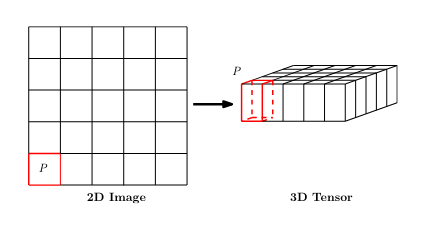
\includegraphics[width=0.8\linewidth]{Figure1.png}
    \caption{Transforming 2D image into 3D tensor}
    \label{Fig1}
  \end{center}
\end{figure}